\documentclass[10pt, a4paper]{article}
\usepackage[english]{Arno}

  \title{Eiosis Test Report}
  \date{\today}
  \bigskip
  \author{\arno}

%##########################################
% START OF THE DOCUMENT
%##########################################
\begin{document}

\maketitle
\bigskip

%**** Logos ****
\vfill
\begin{center}
	
\includegraphics[height=3cm]{images/eiosis-logo.png}
\end{center}


\newpage
%******************************************
%**** Table des matières *****
\tableofcontents




\newpage

\newpage
\section{Test results}

\subsection{Part 1}

\subsubsection{GUI}

\subsubsection*{Final GUI look debate}

This is a part to talk with the client about the final GUI look. It presents the problems which appear in the previous document, and a potential solution to solve it. It also give some development option to solve the problems.

\paragraph*{Problems with previous document}

There is a list of the problems detected, by form of questions (considered answers are marked to explain the solution I have chosen):
\begin{itemize}
	\item Does the panel setting included into an existing panel of plugins, or can it be into a new windows ? (new windows);
	\item Are there an exhaustive list of the settings ? (yes);
	\item Are those setting commons to all plugins, only few of them, none ? (few of them);
	\item How does the user accessing to this panel ? (a button on all the Ul managers).
\end{itemize}

\paragraph*{Possible interface sketch}

A possible GUI is the following:

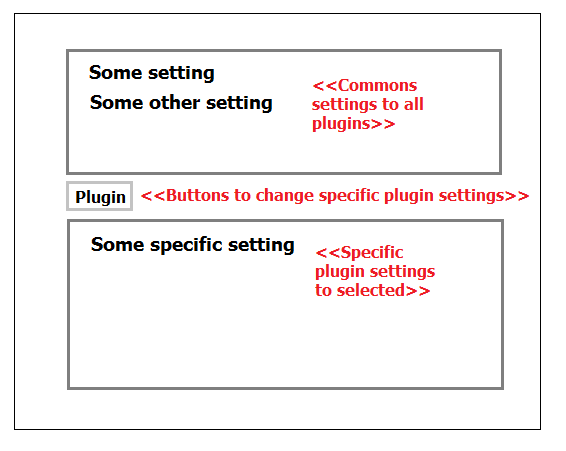
\includegraphics[width=\linewidth]{images/GUI0.png}

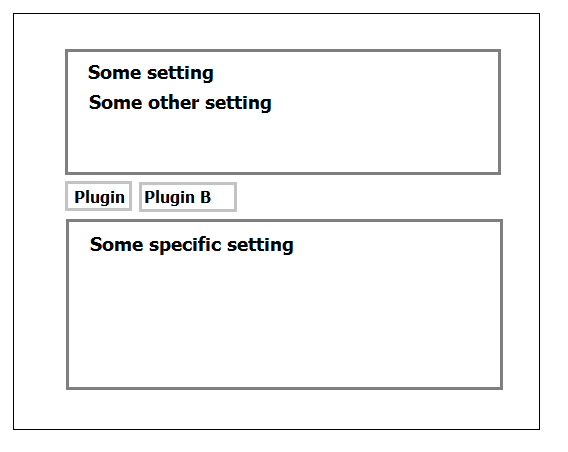
\includegraphics[width=\linewidth]{images/GUI1.png}

\paragraph*{Explanations} 

This solution provides the possibility to define some settings which are commons to all the plugins (displayed on the top, because those are generally the most used). A button could hide/show this part if there are lots of specifics settings.

The list of open plugins allow via a button to change the specific settings to each of the plugin (displayed between both settings parameter, giving clarity). An horizontal scroll bar can appears if a lot of plugins are open. The button only appear once for each instances.

The specific settings of the selected plugin is on bottom, a vertical scroll bar should be needed.

\bigskip
A button will be added to the plugin manager window, to open this panel (and a keyboard short-cut can be added too).

\paragraph*{Why those choices}

By forcing only one instance of this window, I provide the possibility to manage settings easily. I allow to manage the case of plural instances of plugins into the same window (requires static attribute on settings), and plurality of plugins into the same window.

\paragraph*{Events}

Some events are modifying this window:
\begin{itemize}
	\item Load/Save of settings;
	\item Settings change (by user actions);
	\item Launch/Exit of a plugin (add or remove buttons, hide specifics settings, update commons settings to later version);
	\item Update of a plugin (but forcing to exit it solve update change).
\end{itemize}

The save of setting should offers to user the possibility to a previous version of the plugin (see XML part for details) and to cloud the settings (for a company usage for examples (providing the same setting for many customers)).

\paragraph*{Problem raised}

This solution raise a problem, in the case of an update of only a part of the plugin by the user, the common part of the setting shall provide the last version of it (of the launched plugins). Any changes on this part shall provide at least the old settings (accessibility and kind of value) or be hide and force default value.






\subsubsection{The XML file}

To provide retro-compatibility, it is important to start the XML by giving the plugin version. The XML file should not remove any of the previously defined field, to able a previous version of the plugin to load anyway.


\subsubsection{The setting manager}

A setting manager will be a big part of the project, it role will be to manage the events made by the user (via GUI notification), to change the state of the settings, to manage the save and loads, to update the GUI and to update the plugins according to changes.

This manager will also manage a stack of setting state to allow user to cancel and redo some changes.

\subsubsection{The setting state}

The setting state should contains the state of the values given by the GUI (via the setting manager).

According by the fact I have chosen to have a part of this setting common to all the plugins, and the fact of settings are shared by all instance of one plugin: this setting state will be a static object with a common part to all plugins and some specific parts, where each of the specific part are only instantiate once.


\subsubsection{Object diagram}

\begin{changemargin}{-3cm}{-3cm}
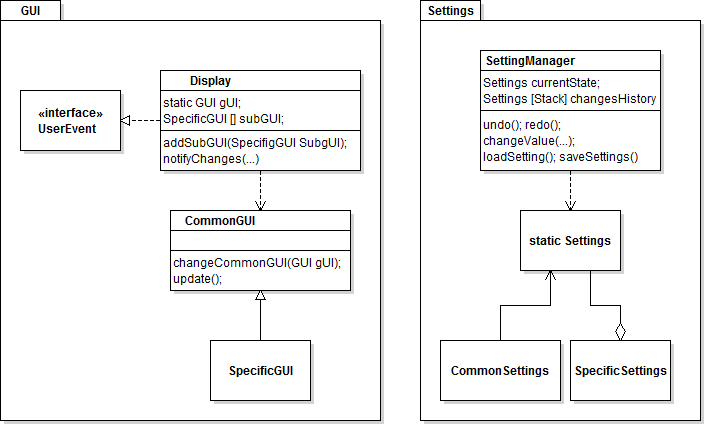
\includegraphics[width=\linewidth]{images/diag1.png}
\end{changemargin}

N.B.: All those elements will be new, the modification required on the existing plugins are only the modification due to the creation of settings for those (if they do not exists yet).


\subsubsection{Comment}

Thanks to the few modifications require on existing plugins, an agile life cycle should be used: the first main step will to make the setting panel for a unique plugin, and other plugin specific panels should be done by the following.

Agile life cycle should works well with the high dependency of the project, the size of the team affected to the project (only few developers) and the global size of the main part of the project.








\newpage
\subsection{Part 2}

The \textbf{Rocky.dll} file is the \textbf{Documents/} folder.\\
For sources, use git repository \textit{https://github.com/ArnaudPanaiotis/Eiosis.git}

\paragraph*{About the bug fix}
~

\bigskip
The bug making Rocky freeze when trying to save or load is now fixed.
\bigskip

The file is written successfully in the wanted repository.
\bigskip

The loading does not set the values displayed to the previous state when saving, a check of specification is required to know if this is supposed to be the normal comportment of those actions.




\newpage
\subsection{Part 3}

 
To give the best feedback related to the asked questions, I write an answer for each of them. 

\paragraph*{is it reliable ?}

Yes, reliability and efficiency are the both quality TUIO team has chosen.

\paragraph*{does it have dependencies or requirements ? which ones ? if yes, could it be a problem ?}

SDL, OpenGL and GLUT libraries are required to build on Mac OS X and Linux system, but this should not create troubles.

The lack of code example and tutorial (even on web) could create difficulty in it usage.

\paragraph*{how do we build it ?}

A Microsoft Visual Studio project is given. Furthermore, a Makefile is given for Linux system. Only library dependency is needed for Mac OS X (SDL, OpenGL and GLUT).

\paragraph*{is it well coded ? what do you think ?}

Yes, classical standards of code implementation are respected, and Doxygen is in use successfully for .h files.

\paragraph*{is it scalable, configurable, tweakable ?}

Yes, according the license \textit{you can redistribute it and/or modify it under the terms of the GNU General Public License as published by the Free Software Foundation}.

\paragraph*{what are its strengths and weaknesses ?}

\subparagraph*{Strengths}

The library is offering a complete set of multi-touching interaction, which allows future evolutions if needed.

It documentation is clear and functions are self-descriptive.

An example of use is given.

Few videos and a well-noted Sourceforge repository are announcing a good library.

\subparagraph*{Weaknesses}

The library should offers to much multi-touch interaction for our requirements (to much code and documentations).

The lack of tutorials and examples could be a problem.


\paragraph*{what about the threading model, is it scalable ?}

The threading model is included into the library and should be scaled.

\paragraph*{is it worth it at the end ?}

I think this library is worth for Eiosis.



\newpage
\section{Feedback}

\subsection{Configuration/ installation issue}

\subsubsection*{Environment}

\paragraph*{Operating system}
\begin{boxedverbatim}
	Windows 7 Professional 64 bits
	Service Pack 1
\end{boxedverbatim}
\paragraph*{IDE version}
\begin{boxedverbatim}
	Microsoft Visual Stidio Premium 2013
	Version 12.0.21005.1 REL
	
	Microsoft .NET Framework
	Version 4.5.50938
\end{boxedverbatim}

\subsubsection*{Description}

After having loaded with success the given version of the project (build\textbackslash all\textbackslash vs2012\textbackslash Eiosis.snl), it raises an error before stating to generate.

This probably come from my version of Microsoft Visual Studio version, which is 2013.

The solution I finally found is to use the vs2010\textbackslash Eiosis.sln project, which generate successfully.

\bigskip
N.B.: This solution should be notify in the given document to provide lost of time to people using Visual Studio 2013. 




\end{document}